\item {\color{red} En el presente trabajo deben realizar la asignación a todos los elementos de la red y realizar su respectiva configuración, de modo que todos los elementos de la red puedan comunicarse entre si. 
\\{ }\\
Deben escribir los comando utilizados en los routers y switches si corresponde en su tarea que sera subida por la plataforma.}\\{ }\\
\noindent
La siguiente configuración de red es la que se realizó utilizando \textit{Cisco Packet Tracer 7.2.2}, en ambos routers el \texttt{Giga0} se conectó al switch y el \texttt{Giga1} entre los routers.

\begin{figure}[ht!]
\centering
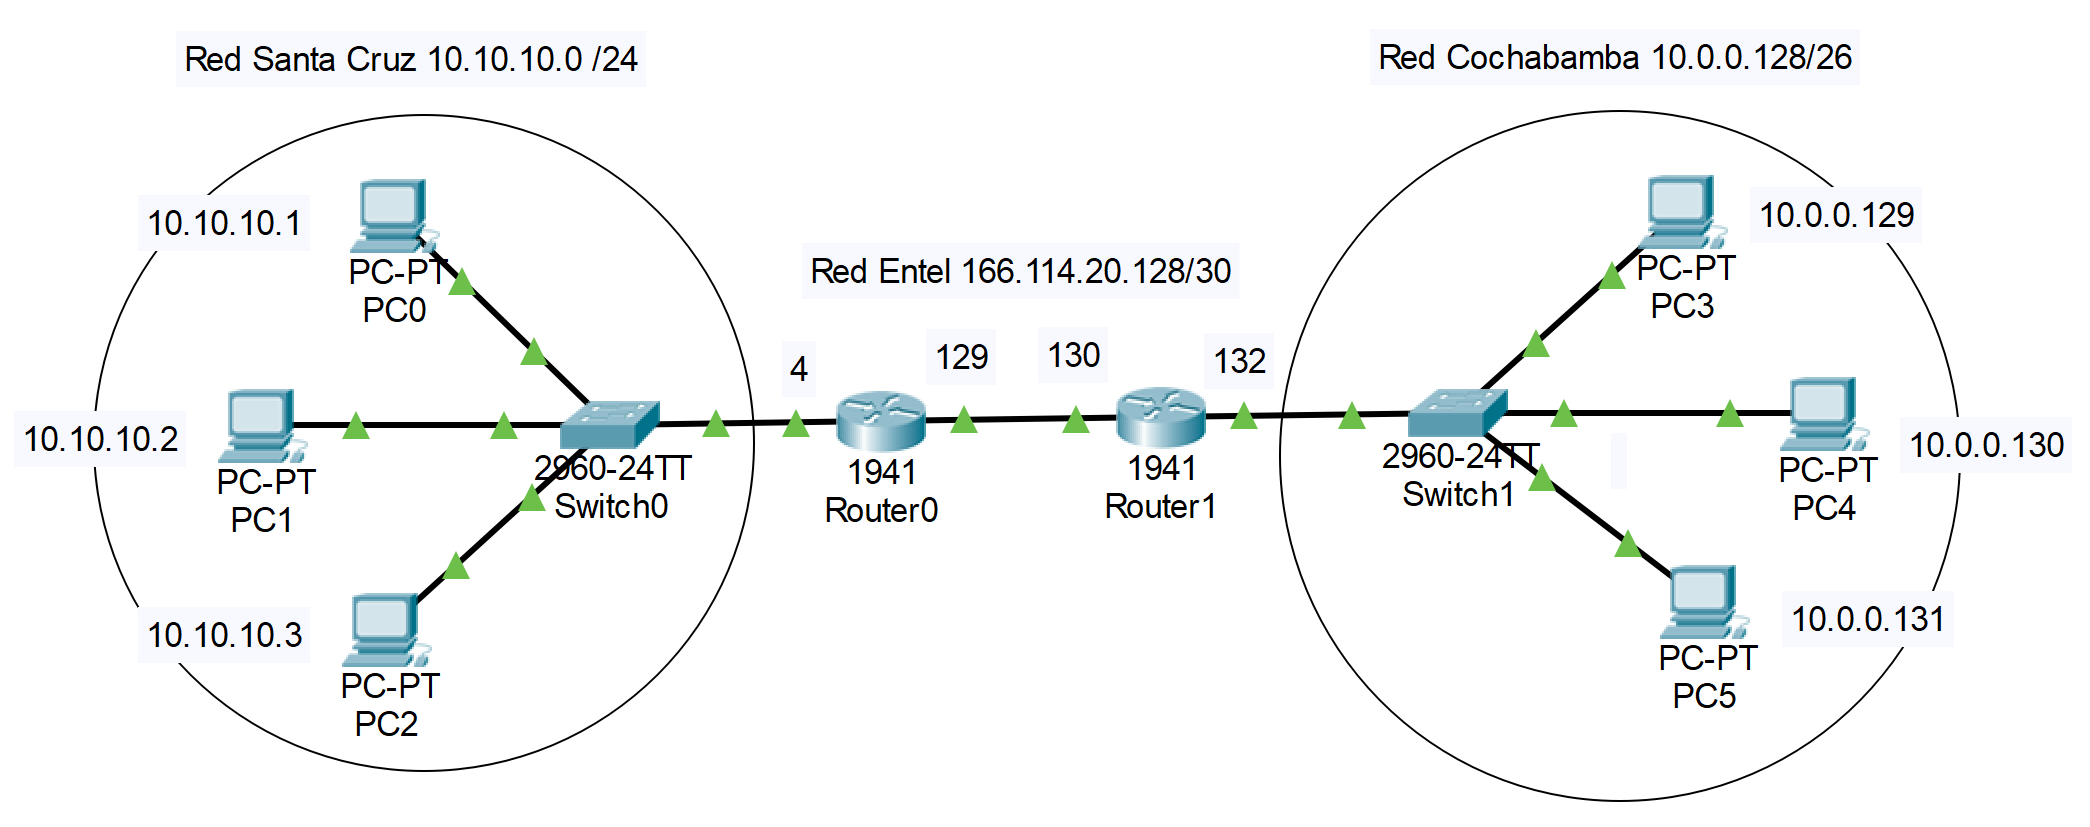
\includegraphics[scale=0.75]{Imagenes/net.png}
\end{figure}
Comandos utilizados para el \texttt{Router0}: \\{ }\\
\texttt{
\noindent
Router\# conf t \\
Router(config)\# int Gig0/0 \\
Router(config-if)\# ip add 10.10.10.4 255.255.255.0 \\
Router(config-if)\# no shut \\
Router(config-if)\# exit \\
Router(config)\# int Gig0/1 \\
Router(config-if)\# ip add 166.114.20.192 255.255.255.252 \\
Router(config-if)\# no shut \\
Router(config-if)\# exit \\
Router(config)\# ip route 10.0.0.128 255.255.255.192 166.114.20.130
}

\pagebreak
Comandos utilizados para el \texttt{Router1}: \\{ }\\
\texttt{
\noindent
Router\# conf t \\
Router(config)\# int Gig0/0 \\
Router(config-if)\# ip add 10.0.0.132 255.255.255.192 \\
Router(config-if)\# no shut \\
Router(config-if)\# exit \\
Router(config)\# int Gig0/1 \\
Router(config-if)\# ip add 166.114.20.130 255.255.255.252 \\
Router(config-if)\# no shut \\
Router(config-if)\# exit \\
Router(config)\# ip route 10.10.10.0 255.255.255.0 166.114.20.129 \\
}

Finalmente, en ambos casos escribimos \texttt{write memory} para guardar las configuraciones.